\documentclass[12pt,a4paper]{article}
\usepackage{etex}
\usepackage[T1]{fontenc}
\usepackage[utf8]{inputenc}
\usepackage[italian]{babel}
\usepackage[a4paper]{geometry}
\usepackage[pdftex]{graphicx}

\usepackage{microtype}
\usepackage{indentfirst}
\usepackage{mathrsfs}
\usepackage{caption}
\usepackage{color}
\usepackage{siunitx}
%

\usepackage{amsmath}
\usepackage{amssymb}
\usepackage{amsfonts}
\usepackage{amsthm}
\usepackage{booktabs}
\usepackage{paralist}
\usepackage{subfig}
\usepackage{array}
\usepackage{xy}
\usepackage{multicol}
%\usepackage{slashbox}
\usepackage{fancyhdr}
\usepackage{makeidx}
\usepackage{hyperref}
\usepackage{wrapfig}
\usepackage[T1,OT1]{fontenc} 
\usepackage{chemfig}
\usepackage{epigraph}
\usepackage{textcomp}
\usepackage[makeroom]{cancel}
\usepackage{enumitem}
\usepackage{braket}

\usepackage{grffile}
\usepackage{tikz}
\usepackage{pgf,tikz}
\usetikzlibrary{shapes.geometric,calc}

\usetikzlibrary{arrows}

\usepackage{mathptmx}
\usepackage[scaled=.90]{helvet}
\usepackage{courier}
\usepackage{mdwlist}

\author{Belliardo Federico \footnote{federico.belliardo@sns.it}}

\title{$\mathbb{Z}_2$ gauged Ising model}

%\title{Seminario d'esame: Transizioni di fase e fenomeni critici}

\begin{document}


\maketitle

\tableofcontents

%TODO
%correggere teorema di elitzur nella parte finale
%modificare derivazione del loop dipendente dal perimetro?

\begin{abstract}
Si svilupperà uno studio della transizione di fase del modello di Ising con simmetria di gauge $\mathbb{Z}_2$ che presenta un parametro d'ordine non locale. Essa potrebbe risultare utile per la comprensione del confinamento dei quarks nella QCD \index{QCD}.
\end{abstract}


\section{Modelli su reticolo e sviluppi in serie}
I modelli su reticolo possono essere studiati utilizzando tre tecniche diverse:

\begin{itemize}
\item simulazioni Monte Carlo, per esempio sfruttando algoritmi di tipo Metropolis.
\item gruppo di rinormalizzazione, con trasformazioni di \emph{blocking} alla Kadanoff.
\item sviluppi in serie ad alta o bassa temperatura.
\end{itemize}

Gli sviluppi in serie in genere considerano un limite risolvibile della teoria (in genere temperatura nulla o infinita) e a questo aggiungono perturbazioni tipicamente rappresentate da una serie di grafi nel reticolo per scrivere la funzione di partizione come serie di potenze in un parametro che  un'opportuna funzione della temperatura. Queste serie posso essere usate per estrapolare la temperatura e gli indici critici i una transizione di fase.
Il fatto che la funzione di partizione sviluppata in serie (per $N$ infinito) abbia un raggio di convergenza finito è indice del fatto che presenti una non analiticità per una temperatura finita e quindi una transizione di fase.
\subsection{Sviluppo a bassa temperatura}
Consideriamo il modello di Ising in $d$ dimensioni:

\begin{equation}
-\beta \mathcal{H} = K \sum_{\left< i, j \right>} \sigma_i \sigma_j
\end{equation}

dove $\sigma_{i} = {+1, -1}$. A bassa temperatura il sistema (in dimensione maggiore di 1) presenta magnetizzazione spontanea. Dobbiamo scegliere uno dei due ground state (tutti spin up o tutti spin down) intorno a cui effettuare il lo sviluppo in serie. Scegliamo $\sigma_i = +1 \quad \forall i$. L'eccitazione di minore energia a partire da questo è un singolo spin \emph{flippato}. Ognuno degli $N$ siti del reticolo può essere scelto per posizionare l'eccitazione, il cui costo energetico è $4Kd$ rispetto al ground state. $2d$ è la connettività del reticolo. L'eccitazione successiva è un dimero di due spin negativi, il quale (trascurando effetti di bordo) h una molteplicità di $Nd$. Infatti scelta la posizione in cui mettere il pirmo spin down vi sono $2d$ modi di mettere il secondo e si deve togliere un fattore $\frac{1}{2}$ per non contare due volte la stessa configurazione. Il dimero ha energia $2 K \left( 4 d -2 \right)$. La successiva eccitazione da considerare sono due spin down separati. Possiamo andare avanti considerando tutte le possibili inserzioni di spin down nel mare di spin up, evidentemente fino ad esaurire le configurazioni del sistema, ottenendo la funzione di partizione completa. E' evidente che l'unico parametro che conta ai fini del bilancio energetico delle ''isole'' di spin che si inseriscono è l'estensione del contorno delle isole in cui si realizza il contatto con gli spin up. La densità dell'eccitazione (rispetto al mare positivo) è concentrata sul suo bordo. Secondo quanto detto abbiamo la rappresentazione:

%TODO Kardar ci mette anche un 2 nell'espressione esatta ma secondo me non ci vuole, lui conta la degenrazione a bassa temperatura, ma non ha senso perchè dovresti solo considerare le fluttuazini attorno al ground state che hai scelto e inoltre la funzione di partizione toale si scrive evidentemente senza il 2.

\begin{equation}
Z = e^{N d K} \sum_{I} e^{- 2 K \times V^{d-1} \left( \partial I \right) }
\end{equation}

dove $I$ è un'isola di spin $\downarrow$, $\partial  I$ ne è il bordo e  $ V^{n-1} \left( \partial I \right)$ ne è il volume $n-1$-dimensionale. I primi termini sono:

\[
Z = e^{N d K} \left[ 1 + N e^{-4 d K} + d N e^{-4 \left( 2 d - 1 \right) K} + \frac{N (N - 2 d -1)}{2} e^{-8 d k} + ... \right]
\]

%TODO Aggungere eventualemnte discussione di Kardar sull'estrapolazione... Come si dimistra che le serie hanno raggio di convergenza finito?

In genere si caratterizza la rottura spontanea di simmetria in questo modello aggiungendo un campo magnetico $h$ che si accoppia agli spin e mostrando che nel limite $N \rightarrow \infty$ $h \rightarrow 0$ si ha un valore medio non nullo per lo spin in una posizione generica $\left< \sigma_i \right>$ a i sotto di una certa temperatura. Notiamo che è impossibile per un numero di finito di spin descritti da una distribuzione di Boltzmann avere una valore di aspettazione non nullo per operatori che rompono la simmetria globale $\mathcal{Z}_2$. Notiamo che rottura di simmetria è in effetti associata ad una rottura dell'ergodicità.


\subsection{Sviluppo ad alta temperatura}
ad alta temperatura gli spin sono di fatto non interagenti e la loro distribuzione di probabilità pesa con un uguale coefficiente ogni possibile realizzazione nell'ensamble, cioè: $p = \frac{1}{2^N}$. Indichiamo con $\left< \quad \right> _ 0$ la media sugli spin non interagenti. Possiamo scrivere:

\begin{equation}
Z = \left< e^{-\beta \mathcal{H}} \right> _ 0 = 1 - \beta \left< \mathcal{H} \right> _ 0 + \frac{\beta^2 \left< \mathcal{H}^2 \right> _ 0}{2} + ... 
\end{equation}

Organizziamo l'espansione in potenze di $\tanh K$, notiamo infatti che:

\[
e^{K \sigma_i \sigma_j} = \frac{e^K + e^{-K}}{2} + \frac{e^K - e^{-K}}{2} \sigma_i \sigma_j = \cosh K \left( 1 + \tanh K  \sigma_i \sigma_j \right)
\]

Sostituiamo nella funzione di partizione:

\begin{equation}
Z = \sum_{ {\sigma_i} } e^{K \sum_{\left< i, j \right>} \sigma_i \sigma_j} = \left( \cosh K \right)^{d N} \sum_{ {\sigma_i} } \prod_{\left< i, j \right>} \left( 1 + t \sigma_i \sigma_j \right) 
\end{equation}

Per ogni coppia $\left< i, j \right>$ abbiamo operato la sostituzione descritta sopra dunque raccogliamo una potenza di $\cosh (K)$ pari al numero di \emph{bonds} nel sistema che è circa $Nd$, trascurando gli effetti d bordo (l'ottica è ovviamente di considerare un limite $N \rightarrow \infty$. Abbiamo introdotto $t = \tanh K$. La produttoria da una somma di $2^{Nd}$ termini. che possono essere rappresentati su un grafico evidenziando i \emph{bonds} che compaiono, come si vede in figura \ref{fig:low}.

\begin{figure}[!htb]
\centering
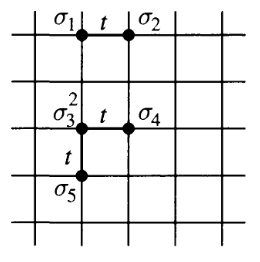
\includegraphics[scale=0.70]{low.png}
\caption{Uno dei termini della sommatoria che da $Z$.\label{fig:low}}
\end{figure}

Ora si opera un'importante semplificazione. Ogni spin compare tante quanti sono i \emph{bond} che si dipartono da lui. Se $p_i$ è questo numero, ogni spin compare in un termine della somma come $\sigma_i ^{p_i}$. Prendendo la sommatoria sugli spin vediamo che sopravvivono solo i termini in cui tutti gli spin hanno esponente pari. Dunque possiamo scrivere $Z$ in termini di una somma tutti i possibili grafici chiusi $\gamma$ che ci possono costruire sul \emph{lattice} (anche intersecanti e autointersecanti).

\begin{equation}
Z = 2^{N} \left( \cosh K \right) ^{N d} \sum_{\gamma} t^{ P(\gamma)} 
\end{equation}

Dove abbiamo indicato con $P(\gamma)$ il perimetro del cammino cioè il numero totale di \emph{bond} di cui è costituito.

\begin{figure}[!htb]
\centering
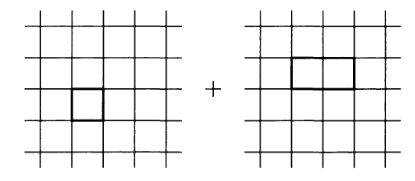
\includegraphics[scale=0.70]{high.png}
\caption{I primo grafici chiusi della serie in $t$.\label{fig:high}}
\end{figure}

I primi termini della serie sono mostrati nella figura \ref{fig:high}. Sono un quadrato formato da quattro collegamenti e un rettangolo (i due quadrati separati hanno perimetro totale maggiore). Un vertice del quadrato può essere scelto in $N$ modi sul reticolo e la sua orientazione in $\frac{d(d-1)}{2}$. Il fattore $2^{N}$ viene dalla somma su tutte le configurazioni di spin.

%TODO Ricavare il fattore combinario per il circutio rettangolare
\[
Z = 2^N  \cosh ^{d N} K \left[ 1 + \frac{d(d-1) N}{2} t^4 + d(d-1)(2d -3) N t ^6\right]
\]

Questa rappresentazione della funzione di partizione permettere anche di risolvere agilmente il modello di Ising in 1D. In una dimensione infatti non ho percorsi chiusi e $Z = 2^N \left( \cosh K \right) ^{N}$.

\section{Somma sui ``polimeri fantasma"}

Abbiamo ottenuto nella sezione precedente che è possibile scrivere la funzione di partizione del modello di Ising come:

\[
Z = 2^N \cosh^{dN} K \times S
\]

dove $S$ è la somma su tutti i grafi chiusi costruibili con i \emph{link} del reticolo. 


\begin{figure}[!htb]
\centering
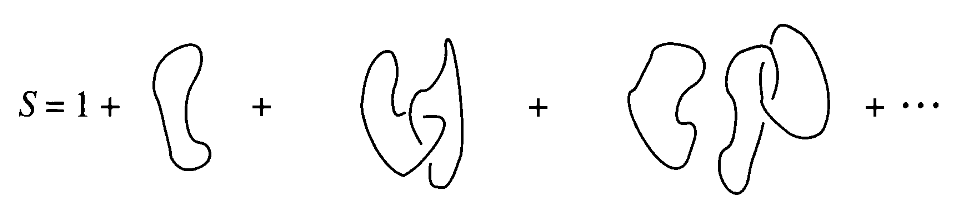
\includegraphics[scale=0.30]{loop.png}
\label{fig:loop}
\end{figure}

Questa formula è suggestiva perché ci ricorda i grafici di Feynman, vediamo se l'analogia si può estendere ulteriormente. Indichiamo con $\Theta$ la somma di tutti i percorsi chiusi a 1 loop non autointersecanti. Definiamo: \[S' = e^{\Theta} = 1 + \Theta + \frac{1}{2} \left( \Theta \right)^2 + \frac{1}{6} \left( \Theta \right)^3 + ... \]

La potenza $n$-esima nell'espansione sovrappone $n$ loop, anche intersecandoli o contando un singolo link più volte. Per questa ragione non può essere $S = S'$, cioè in $S'$ ci sono termini che non esistono in $S$ come quelli nella figura \ref{fig:termini}.

\begin{figure}[!htb]
\centering
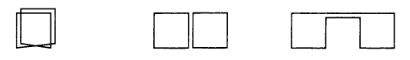
\includegraphics[scale=0.50]{termini.png}
\caption{Alcuni termini presenti in $S'$ che sono assenti in $S$.\label{fig:termini}}
\end{figure}

In effetti possiamo interpretare $S$ come la funzione di partizione di un gas di polimeri che possono intersecarsi ma non occupare link già presi, mentre $S'$ è un gas di polimeri ''fantasma'' che possono occupare link già presi da altri.

Consideriamo la funzione di correlazione a due punti $\left< \sigma_0 \sigma_{\mathbb{r}} \right>$ per la funzione di partizione $S'$, è possibile dimostrare che essa è la somma di tutti i contributi da 0 a $\mathbb{r}$.

\begin{figure}[!htb]
\centering
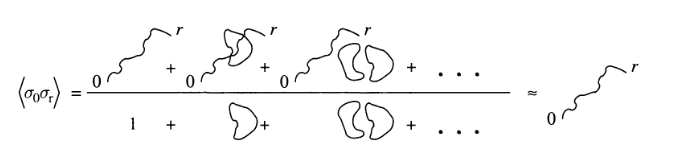
\includegraphics[scale=0.60]{corr.png}
\caption{Forma suggestiva della funzione di correlazione per $S'$.\label{fig:corr}}
\end{figure}

Inoltre la funzione $S'$ si può risolvere esattamente e mostrare che riproduce i risultati della teoria gaussiana. 

\section{Dualità di Kramers-Wannier}

E' noto che il confronto delle due serie per il modello di Ising bidimensionale produce la dualità di Kramer-Wannier che permette di trovare il valore esatto della temperatura critica in 2 dimensioni. Riscriviamo i primi termini delle 2 serie in 2D:

\[
Z = e^{2 N K} \left[ 1+ N e^{-4 \times 2 K} + 2 N e^{-6 \times 2K} + ...\right] 
\]

\[
Z = 2^N \cosh^{2N} K \left[ 1 + N \tanh^4 K + 2 N \tanh^6 K + ... \right]
\]

Se indichiamo con $g(x) = \frac{1}{N} \ln \left( 1 + N x^4 + 2 N x^6 + ... \right)$ abbiamo che vale la seguente relazione di dualità:

\begin{equation}
2 K + g \left( e^{-2 K} \right) = \ln 2 + 2 \ln \cosh(K) + g(\tanh K)
\end{equation}

Assumiamo che esista un solo punto critico, allora nel limite $N \rightarrow \infty$ sviluppa un solo punto di non analiticità. Se il membro sinistro (come funzione di $K$) è in un punto di non analiticità allora lo è anche il membro sinistro (perché sono la stessa funzione) ma l'unica sorgente di non analiticità può essere la funzione $g$ in quanto  $\ln \cosh(K)$ è analitica (si scrive come serie di potenze convergente in un intorno), quindi $g$ nel membro destro si deve trovare al punto critico. Esso si trova a $e^{-2 K} = \tanh (K)$.

\section{$\mathbb{Z}_2$ gauged Ising model}
Possiamo chiederci analogamente se esiste una relazione di dualità per il modello di Ising in 3D, scriviamo le due serie corrispondenti:

\[
Z = e^{3 N K} \left[ 1 + N e^{- 2K \times 6} + 3 N e^{-2K \times 10} + ... \right]
\]

\[
Z = 2^N \cosh^{3N} K \left[ 1 + 3 N \tanh^4 K + 18 N \tanh^6 K + ... \right]
\]

Le due somme sono differenti e in 3D il modello di Ising non è duale a se stesso. Possiamo chiederci però se esiste un'Hamiltoniana la cui serie ad alta temperatura riproduce la serie a bassa temperatura del modello di Ising. Un simile modello esiste ed è il seguente:

\begin{equation}
-\beta \mathcal{H} = \tilde{K} \sum_{P} \tilde{\sigma}_P^1 \tilde{\sigma}_P^2 \tilde{\sigma}_P^3 \tilde{\sigma}_P^4
\end{equation}

Immaginiamo di inserire uno spin su ogni link del reticolo tridimensionale. Allora chiamiamo \emph{plaquette} un quadratino elementare costituito da 4 link adiacenti. L'Hamiltoniana di sopra è costruita sommando su tutte le \emph{plaquette} del reticolo il prodotto dei quattro spin sopra di essa. La costante di accoppiamento $\tilde{K}$ è definita come:

\begin{equation}
\tilde{K} = -\frac{1}{2} \ln \tanh \left( K \right)
\end{equation}

Vediamo che abbiamo realizzato al dualità. Possiamo scrivere un espansione ad alta temperatura per il nostro modello:

\begin{equation}
Z = \cosh^{3N} ( \tilde{K} )  \sum_{ {\sigma_P^i = \pm 1}} = \prod_{P} \left( 1 + \tanh \tilde{K} \tilde{\sigma}_P^1 \tilde{\sigma}_P^2 \tilde{\sigma}_P^3 \tilde{\sigma}_P^4 \right)
\end{equation}

L'esponente $3N$ viene dal numero di \emph{plaquette} che si trovano in un reticolo 3D. Svolgendo la produttoria troviamo la somma di $2^{3N}$ termini ognuno dei quali contribuisce solamente se ogni spin compare con un esponente pari. In caso contrario la sommatoria su tutte le configurazioni degli spin eliminerà il termine corrispondente. 
I termini che contribuiscono sono pertanto solamente quelli le cui \emph{plaquette} formano volumi chiusi nello spazio 3D (non necessariamente connessi). Il numero di \emph{plaquette} che costituiscono la superficie è proprio il numero di spin che contribuiscono all'energia di un isola di spin $\downarrow$ in un mare di spin $\uparrow$. La superficie è proprio l'esponente di $\tanh \tilde{K}$ nello sviluppo in serie. 

Dunque scriviamo:


\[
Z = 2^N \cosh^{3N} ( \tilde{K} ) \sum_{I} \left[ \tanh(\tilde{K}) \right] ^ {A(\partial I)} =  2^N \cosh^{3N} ( \tilde{K} ) \sum_{I} e^{-2 K \times A(\partial I)}
\]

dove $A(\partial I)$ è l'area dell'isola di spin $I$ (in 3D). Dunque a meno di funzioni regolari si può scrivere l'energia libera per spin di questo modello che chiameremo $\mathbb{Z}_2$ gauged Ising model in termini dell'energia libera di un modello di Ising 3D. Dunque questo modello deve presentare una transizione di fase e l'indice critico del calore specifico deve essere uguale a Ising 3D.

Ci possiamo accorgere che il modello presenta un gruppo di simmetria ben più ampio del normale modello di Ising. Per quest'ultimo è possibile \emph{flippare} tutti gli spin contemporaneamente e mantenere invariata l'Hamiltoniana. A causa dell'accoppiamento con i primi vicini non è possibile \emph{flippare} un numero limitato di spin localmente e mantenere invariata l'energia perché i bordi della regione su cui operiamo contribuiranno sempre a dare una differenza di energia. Il modello di Ising è detto avere simmetria $\mathbb{Z}_2$

Se consideriamo invece il $\mathbb{Z}_2$ gauged Ising model vediamo che è possibile flippare i 6 spin attorno a una posizione $n$ nel reticolo senza cambiare l'energia, infatti ogni \emph{plaquette} avente $n$ come vertice conterrà il prodotto di due di questi spin. 

\begin{figure}[!htb]
\centering
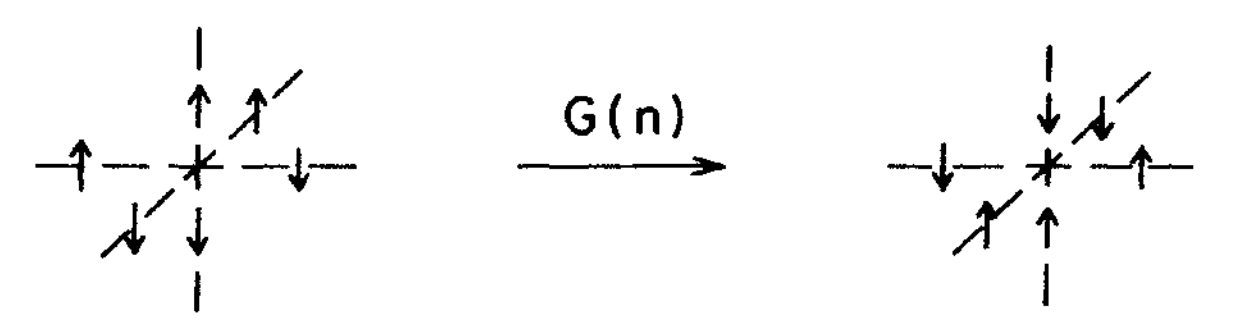
\includegraphics[scale=0.20]{gauge.png}
\caption{Trasformazione di gauge del modello $\mathbb{Z}_2$ gauged Ising.\label{fig:gauge}}
\end{figure}

Il modello ha pertanto una simmetria locale molto più grande del modello di Ising. Questa è chiamata simmetria di gauge in analogia con la fisica delle interazioni fondamentali.

\section{Dualità in altre dimensioni}
Ci potremmo chiedere perché non abbiamo trovato questa dualità in dimensione 2 e se l'abbiamo in dimensione superiore. La dualità esiste in più dimensioni se si considerano ipercubi a $d-1$ dimensioni invece di \emph{plaquette} e si somma il prodotto degli spin su tutti i possibili ipercubi del reticolo. I termini che sopravvivono sono le ipersuperfici che incapsulano una o più isole di spin, esattamente come in 3D. Anche in alte dimensioni il modello ha una simmetria locale, essa è data dalla possibilità di \emph{flippare} i $2d$ spin sui link che si dipartono da un certo vertice. Perché in 2D non l'abbiamo trovata? L'equivalente in 2D delle \emph{plaquette} sono i link singoli e ognuno di essi possiede un solo spin... finire.

\section{Il teorema di Elitzur}
Siamo interessati a studiare la transizione di fase di questo modello e per farlo dobbiamo individuare il parametro d'ordine. Anticipiamo che questo non può essere la magnetizzazione (né nessun altra funzione di correlazione non gauge invariante).
Vogliamo verificare se si verifica magnetizzazione spontanea a bassa temperatura, per farlo introduciamo un termine che rompe esplicitamente la simmetria $\mathbb{Z}_2$ e verifichiamo se persiste una magnetizzazione anche mandandolo a 0 (nel limite termodinamico).

\begin{equation}
-\beta \mathcal{H} = \tilde{K} \sum_{P} \tilde{\sigma}_P^1 \tilde{\sigma}_P^2 \tilde{\sigma}_P^3 \tilde{\sigma}_P^4 + h \sum_{i} \tilde{\sigma_i}
\end{equation}

Calcoliamo:

\begin{equation}
\left< \tilde{\sigma}_n \right> = \frac{\sum_{ {\tilde{\sigma}_i = \pm 1}} \tilde{\sigma}_n e^{\tilde{K} \sum_{P} \tilde{\sigma}_P^1 \tilde{\sigma}_P^2 \tilde{\sigma}_P^3 \tilde{\sigma}_P^4 + h \sum_{i} \tilde{\sigma_i}}}{ \sum_{ {\tilde{\sigma}_i = \pm 1}} e^{\tilde{K} \sum_{P} \tilde{\sigma}_P^1 \tilde{\sigma}_P^2 \tilde{\sigma}_P^3 \tilde{\sigma}_P^4 + h \sum_{i} \tilde{\sigma_i}}
}
\end{equation}

Supponiamo di aver già effettuato il limite $N \rightarrow \infty$, mostreremo che questo valore di aspettazione si annulla per $h \rightarrow 0$ e per farlo sfrutteremo l'invarianza di gauge locale del modello. Consideriamo uno dei due vertici a cui è collegato lo spin in posizione $n$ ed eseguiamo una trasformazione di gauge sui $2d$ vertici adiacenti. Chiamo $\lbrace l_n \rbrace$ questi spin e $\tilde{\sigma}'$ le variabili \emph{flippate}. Allora possiamo scrivere le variabili vecchie in funzione di quelle nuove aggiungendo una variazione dello spin che è diversa da 0 solo nella regione in cui ho eseguito il \emph{flip}.

\begin{equation}
\tilde{\sigma}'_i = \tilde{\sigma}_i + \delta \tilde{\sigma}_i
\end{equation}

dove $\delta \tilde{\sigma} = - 2 \tilde{\sigma} = 2 \tilde{\sigma}'$ se $i \in \lbrace l_n \rbrace$ e $\delta \tilde{\sigma} = 0$ altrimenti. Sostituendo nel valore di aspettazione di sopra abbiamo:

\[
\left< \tilde{\sigma}_n \right> = - \frac{1}{Z}\sum_{ {\tilde{\sigma}_i = \pm 1}} \tilde{\sigma}'_n e^{\tilde{K} \sum_{P} \tilde{\sigma}_P'^1 \tilde{\sigma}_P'^2 \tilde{\sigma}_P'^3 \tilde{\sigma}_P'^4 + h \sum_{i} \tilde{\sigma}'_i + h \sum_{i} \delta \tilde{\sigma}_i} =  - \frac{1}{Z}\sum_{ {\tilde{\sigma}_i = \pm 1}} \tilde{\sigma}'_n  e^{+ h \sum_{i} \delta \tilde{\sigma}_i}  e^{\tilde{K} \sum_{P} \tilde{\sigma}_P'^1 \tilde{\sigma}_P'^2 \tilde{\sigma}_P'^3 \tilde{\sigma}_P'^4 + h \sum_{i} \tilde{\sigma}'_i}
\]

La somma su tutte le configurazioni di spin $\lbrace \tilde{\sigma}_i = \pm 1 \rbrace$, si può sostituire con la somma su tutte le configurazioni $\lbrace \tilde{\sigma}'_i = \pm 1 \rbrace$ visto che stiamo comunque considerando tutte le possibilità, solo in un ordine diverso. E' inoltre evidente che nella funzione di partizione possiamo rinominare le variabili di spin:

\[
Z = \sum_{ {\tilde{\sigma}_i = \pm 1}} e^{\tilde{K} \sum_{P} \tilde{\sigma}_P^1 \tilde{\sigma}_P^2 \tilde{\sigma}_P^3 \tilde{\sigma}_P^4 + h \sum_{i} \tilde{\sigma_i}} = \sum_{ {\tilde{\sigma}'_i = \pm 1}} e^{\tilde{K} \sum_{P} \tilde{\sigma}_P'^1 \tilde{\sigma}_P'^2 \tilde{\sigma}_P'^3 \tilde{\sigma}_P'^4 + h \sum_{i} \tilde{\sigma_i}'}
\]

Dunque abbiamo:

\[
\left< \tilde{\sigma}_n \right> = - \left< \tilde{\sigma}'_n e^{+ h \sum_{i} \delta \tilde{\sigma}_i} \right> = - \left< \tilde{\sigma}'_n e^{+ h \sum_{i} + 2 \tilde{\sigma}'_i \chi( \lbrace l_n \rbrace )} \right>
\]

La media è fatta sulla distribuzione di spin in cui è presente un campo magnetico $h$. E' a questo punto evidente che nel membro di destra (sia a numeratore che a denominatore) possiamo sopprimere l'apice. Il significato di $\chi( \lbrace l_n \rbrace )$ è di selezionare solamente i $2d$ link prossimi a $\tilde{\sigma}_n$ su cui si era eseguita la trasformazione di gauge. Sopprimiamo gli indici:

\begin{equation}
\left< \tilde{\sigma}_n \right> = \left< - \tilde{\sigma}_n e^{+ h \sum_{i} + 2 \tilde{\sigma}_i \chi( \lbrace l_n \rbrace )} \right>
\end{equation}

Da questo possiamo ottenere una stima per $|\langle \tilde{\sigma}_n \rangle |$:

\[
2 |\langle \tilde{\sigma}_n \rangle | = | \langle \tilde{\sigma}_n \rangle - \langle - \tilde{\sigma}_n \rangle| = \left| \left< - \tilde{\sigma}_n e^{+ h \sum_{i} + 2 \tilde{\sigma}_i \chi( \lbrace l_n \rbrace )} \right> - \langle - \tilde{\sigma}_n \rangle \right| = 
\]

\[
= \left| \left< - \tilde{\sigma}_n \left[ e^{+ h \sum_{i} + 2 \tilde{\sigma}_i \chi( \lbrace l_n \rbrace )} - 1 \right] \right> \right| \leq \left| e^{4 d h} - 1 \right| \left| \left<  \tilde{\sigma}_n \right> \right| 
\]

I ognuno dei termini della somma che costituiscono la media termica si può utilizzare una disuguaglianza che deriva dl fatto che la sommatoria a esponente è ristretta a $2d$ link che possono valere al massimo 2:

\[
e^{+ h \sum_{i} + 2 \tilde{\sigma}_i \chi( \lbrace l_n \rbrace )} - 1 \leq e^{4dh} - 1
\]

scrivendo cioè:

\[
\frac{1}{Z} \sum \tilde{\sigma}_n \left[ e^{+ h \sum_{i} + 2 \tilde{\sigma}_i \chi( \lbrace l_n \rbrace )} - 1 \right] e^{\beta \mathcal{H}} \leq \left( e^{4dh} - 1 \right) \frac{1}{Z} \sum \tilde{\sigma} e^{\beta \mathcal{H}} = \left( e^{4dh} - 1 \right) \left< \tilde{\sigma} \right>
\]

Per poter passare al valore assoluto la disuguaglianza dobbiamo assumere che entrambi i membri siano positivi, cosa vera poiché $h \geq 0$ favorisce gli spin nella direzione positiva, dunque ricaviamo la disuguaglianza:

\[
2 |\langle \tilde{\sigma}_n \rangle | \leq  \left( e^{4 d h} - 1 \right) \left| \left<  \tilde{\sigma}_n \right> \right| 
\]

\textbf{ATTENZIONE}: C'è qualcosa che non va e questa disuguaglianza in questa formula che non può essere giusta...


Abbiamo appena mostrato che non vi può essere magnetizzazione spontanea a qualsiasi temperatura (che è entrata come costante moltiplicativa in $\tilde{K}$ e $h$). In effetti è intuitivo capire il perché. Nella fase a simmetria rotta del modello di Ising muoversi da un ground state all'altro richiede la creazione di un'isola di spin di segno opposto che cresce fino a  ``inghiottire" tutto il sistema, ma questo non è energeticamente favorito, in quanto ci è un costo alla creazione di queste isole che scala come la superficie, che per passare all'altro ground state dovrebbe diventare infinita.
Nel modello che abbiamo analizzato è possibile \emph{flippare} tutti gli spin in una regione chiusa senza cambiare l'energia della configurazione dunque non i aspettiamo di avere una fse a simmetria rotta in quanto non vi è nessuna penalità energetica per un isola di spin fluttuanti di dimensione arbitraria. Per realizzare quanto detto è sufficiente \emph{flippare} i $2d$ spin di un vertice ogni due su ogni linea.

Il risultato ottenuto è simile a quello che vieta la magnetizzazione del modello XY a qualunque temperatura derivante dal teorema di Mermin-Wagner.

\section{Simmetria di gauge?}
Abbiamo chiamato questa simmetria aggiuntiva ``di gauge" per significare che si tratta di una simmetria locale. In fisica con simmetria di gauge si intende in genere la possibilità di avere più vettori dello spazio di Hilbert che rappresentano lo stesso stato fisico, dunque avere una ridondanza nella descrizione. Qui non lo stiamo intendendo in questo senso ma solo nel senso che esiste na simmetria locale. In effetto se identificassi le configurazione di spin separati da una delle nostre trasformazioni di gauge non avrebbe proprio senso considerare il valore il valore di aspettazione di operatori non gauge invarianti come $\left< \tilde{\sigma} \right>$.

\textbf{SCRIVERE MEGLIO!!!}
Identificare gli stati fisici a meno di una trasformazione locale di gauge porta solo ad aggiungere una costante moltilicativa nella funzione di partizione. Dunque sommare solo sugli stati fisici (come di fa per calcolare la funzione di partizione in teoria di gauge) porta solo a ridefinire $Z$ a meno di una costante.

\section{Introduzione dei Wilson loop}

Dalla dualità con il modello di Ising 3D sappiamo che la funzione di partizione ha una non analiticità ad una temperatura finita e un discontinuità nella derivata seconda dell'energia libera (quindi nel calore specifico). Ci aspettiamo una transizione di fase dunque al punto di non analiticità di $Z$ ma abbiamo appena visto che $\tilde{\sigma}$ no può essere un parametro d'ordine.
In effetti sostituendo a $\tilde{\sigma}$ un qualunque operatore non gauge invariante nella dimostrazione di sopra si vede che il suo valore di aspettazione è nullo nel limite $h \rightarrow 0$. 

Esiste un'altra transizione di fase nella fisica che non manifesta un parametro d'ordine locale ed è la transizione di fase di BKT nel modello XY. In quel caso abbiamo il teorema di Mermin-Wagner che ci proibisce di avere magnetizzazione spontanea a temperatura finita. In quel caso l'evidenza che vi deve essere essere una transizione di fase viene dall'analisi della funzione di correlazione. Sappiamo che a bassa temperatura essa si comporta come:

\[
\langle \mathbf{S}(\mathbf{r}) \cdot \mathbf{S}(0) \rangle \propto r^{-\frac{k_B T}{2 \pi J}}
\]

mentre ad alta temperatura abbiamo:

\[
\langle \mathbf{S}(\mathbf{r}) \cdot \mathbf{S}(0) \rangle \propto e^{-\frac{r}{\xi}}
\]

Dunque a bassa temperatura la lunghezza di correlazione è infinita e vi deve essere un punto di transizione di fase in cui diventa tale. 
Analizziamo analogamente le funzioni di correlazione a più punti guage invariante:

\begin{equation}
C_{\gamma}= \left< \prod_{\gamma} \tilde{\sigma} \right>
\end{equation}

Cioè consideriamo il prodotto degli spin longo un percorso chiuso. Questo prodotto è l'analogo dei loop di Wilson nelle teorie di campo con simmetria di gauge. 

\textbf{TODO}: Scrivere espressione del loop di Wilson come è nella teoria di Gauge.

Cerchiamo di studiare il comportamento ad alta e bassa temperatura di questo loop.

\section{Tensione di stringa come parametro d'ordine non locale}
Mostreremo che la funzione di correlazione $C_{\gamma}$ ha due comportamenti qualitativamente diversi ad alta e bassa temperatura. Ad alta temperatura essa dipende dall'area della superficie minore che ha come contorno il loop $\gamma$, mentre a bassa temperatura essa dipende dal perimetro del loop. 

\subsection{Andamento ad alta temperatura}
Utilizziamo la rappresentazione ad alta temperatura della funzione di partizione per svolgere questo calcolo.

\begin{equation}
C_{\gamma} = \frac{1}{Z} \sum_{ \lbrace \tilde{\sigma}_i = \pm 1 \rbrace } \left( \prod_{\gamma} \tilde{\sigma} \right)  e^{\tilde{K} \sum_{P} \tilde{\sigma}_P^1 \tilde{\sigma}_P^2 \tilde{\sigma}_P^3 \tilde{\sigma}_P^4}  
\end{equation}

Gli unici termini che contribuiscono al valore di aspettazione dopo aver risolto la sommatoria sugli spin sono quelli in cui ogni spin compare con una potenza pari, questo significa che ogni termine non nullo della somma è in corrispondenza con una superficie che ha come contorno la curva $\gamma$, dunque possiamo scrivere:

\begin{equation}
C = \frac{2^N \cosh^{3 N}}{Z}  \left( \tilde{K} \right) \sum_{\partial S = \gamma} \tanh  ^{V_{d-1}(S)} \left( \tilde{K} \right)
\end{equation}

dove la somma è fatta su tutte le superfici che hanno come contorno $\gamma$. L'estensione della superficie compare a esponente della tangente iperbolica. Ad alta temperatura contano solamente le prime potenze dello sviluppo quindi in particolare solo la superficie di area minima. Otteniamo così:

\begin{equation}
C_{\gamma} \propto e^{-f(\tilde{K}) A}
\end{equation}

dove $f(\tilde{K})$ è una funzione (non importate) di $\tilde{K}$ e $A$ è l'area minima citata sopra.

\subsection{Andamento a bassa temperatura}
Utilizziamo ora lo sviluppo a bassa temperatura per caratterizzare in questo limite la funzione $C_{\gamma}$. A differenza del modello di Ising qui abbiamo un'enorme degenerazione del ground state. Nella fase a simmetria rotta di Ising si verifica una rottura dell'ergodicità così che è possibile calcolare le quantità termodinamiche considerando le fluttuazioni termiche intorno ad uno dei due ground state scelti poiché non è mai possibile avere una fluttuazione termica tanto forte da flippare gli spin. In questo modello invece i ground state non sono separati da alcun costo energetico cosicché per fare lo sviluppo a bassa temperatura bisogna considerare tutti i ground state degeneri legati da quella che abbiamo chiamato una trasformazione di gauge.

Se stiamo calcolando valori di aspettazione di quantità gauge-invarianti sappiamo che avere i ground state degeneri introduce semplicemente una molteplicità. Se abbiamo $N$ vertici nel reticolo questa molteplicità è $2^N$ e si cancella a numeratore e a denominatore.

In sostanza in questo tipo sviluppo stiamo considerando le prime eccitazioni su tutti gli equamente possibili ground state di questo modello per i quali ripetiamo ci aspettiamo che valga l'ipotesi di ergodicità perché non separati da nessuna barriera energetica. L'eccitazione più semplice è il \emph{flip} di uno spin che causa la frustrazione di $2(d-1)$ (nel senso che non sono nello stato energetico più basso). Possiamo scegliere la posizione dello spin da flippare tra tutti i possibili $dN$ spigoli del reticolo.
Inoltre notiamo che nel caso in cui lo spin flippato sia contenuto nella stringa raccolta lungo il percorso $\gamma$ il contributo nel termine nella somma è negativo, mentre è positivo in tuti gli altri casi.

Trascuriamo eccitazioni superiori sul ground state. Per le quali vale sempre l'idea di prendere un rappresentante della classe delle configurazioni di spin invarianti per questa simmetria, considerare le eccitazioni su di esso e la molteplicità. Così si evita di contare più volte una stessa configurazione.  

%NON ACCONTENTARSI DI QUESTO MA METTERE ANCHE ALTR ECCITAZIONI.

Scriviamo dunque il valore di aspettazione
\begin{equation}
C_{\gamma} = \frac{2^{N} e^{\tilde{K} N d} \left( 1 + \left( dN - 2P(\gamma) \right) e^{-4 (d-1) \tilde{K} + ...} \right) }{2^{N} e^{\tilde{K} N d} \left( 1 + dN e^{-4 (d-1) \tilde{K}} + ... \right)} \sim 1 - 2P(\gamma) e^{-4 (d-1) \tilde{K}} + ... \sim e^{-g(\tilde{K}) P(\gamma)}
\end{equation}

Si possono anche sommare i termini in cui si \emph{flippano} altri spin e il risultato non cambia. 

%TODO Aggiungere

Il comportamento diverso della funzione di correlazione segnale la presenza di una transizione di fase associata alla discontinuità che sappiamo esistere per via della dualità con Ising 3D

\section{Tensione di stringa come parametro d'ordine}

Possiamo pensare di introdurre un parametro d'ordine sfruttando questa differenza di comportamento. Definiamo quindi la tensione di stringa:

\begin{equation}
\sigma = - \lim_{A(\gamma) \rightarrow \infty} \frac{\ln C_{\gamma} }{ A(\gamma)}
\end{equation}

calcolata su cammino $\gamma$ sufficientemente regolare la cui area scala come il quadrato delle dimensioni lineari. Questo parametro è nullo a bassa temperatura ed è diverso da zero ad alta.  Ci possiamo immaginare che esso manifesti una non analiticità al punto critico. Questo andrebbe verificato o mediante uno studio della convergenza o delle o mediante metodi numerici. 
Esiste anche un altro oggetto che costituisce un parametro d'ordine... finire di parlare dell'operatore disordine...

\section{Conclusioni}
Senza entrare troppo nei dettagli la fase il cui il loop di Wilson dipende dall'area corrisponde alla fase confinata della QCD, mentre quella in cui la funzione di correlazione dipende dal perimetro del loop corrisponde alla fase deconfinata. Lo studio di questo \textit{toy model} può costituire un laboratorio teorico per studiare questa transizione di fase e costruire un gruppo di rinormalizzazione. 

\begin{itemize}
\item Approfondire il collegamento con le teorie di gauge su reticolo e mostrare che la QED non ha questa transione di fase. 
\item Scrivere qualcosa su un possibile gruppo di rinormalizzazione alla Migdal-Kadanoff.
\item Provare almeno ad approcciare un gruppo di rinormalizzazione per questo modello di Ising.
\item Aggiungere la materia (variabili di ising che possono anche essere numeri di Grassmann) e mostrare come si può provare a indovinare il diagramma di fase.
\item Approfondire relazione con teorie di gauge su reticolo con gruppi più complicati.
\item Aggiungere esplicitamento il collegamento con la QCD e citare il metodo di rinormalizzazione alla Migdal e asserire che non funziona bene. 
\item Scrivere molte cose sulle teorie su reticolo, esplicitare la rotazione di Wick, la discretizzazione, l'argomento QCD per la tensione di stringa. 
\item Dire che usando il gruppo U(1) si può mostrare che gli sviluppi ad alta temperura danno per la QED semmpre una legge di area. Quindi conta il fatto che il gruppo è abeliano ma è anche importante il fatto che sia discret, infatti Z2 ha la transione.
\item Non hanno parametro d'ordine locale, ma hanno la tensione di stringa (che è non locale).
\end{itemize}

\begin{thebibliography}{99} % Beamer does not support BibTeX so references must be inserted manually as below

%\bibitem https://arxiv.org/pdf/1109.3128.pdf
%\bibitem Quantum metrology and its application in biology
%\bibitem https://arxiv.org/pdf/1405.4878.pdf

\bibitem -Kardar - Statistical Field Theory
\bibitem -Kogut - An introduction to lattice gauge theory and spin systems

\end{thebibliography}

\clearpage
\printindex

\end{document}